\subsection{Rahmenbedingungen}
\textit{(pro)} Die in diesem Unterkapitel beschriebenen Rahmenbedingungen sollen die Aufgabenstellung präzisieren und auf den Umgang mit diesem Projekt verwendeten Materialien aus dem Agrar-Bereich sensibilisieren.

\subsubsection{NemaCaps}
Die geometrischen Abmessungen der Nemacaps sind entscheiden, da sie während des Setzprozesses vereinzelt und transportiert werden müssen. Die Abmessungen der Nemacaps wurden deshalb vom Hersteller MCC Laboratoire Meiners mit 3mm Durchmesser und einer Toleranz von +0.6mm spezifiziert. Von Bedeutung ist ausserdem das Alter und die Lagerung der Nemacaps. Sie müssen in einem geschlossenen Gefäss, unter Beigabe eines hygrophoben Pulvers bei unter 7°C gelagert werden. Dabei sollten sie zur Zeit der Verwendung nicht älter als 4 Wochen sein. Nemacaps welche längere Zeit an der Umgebungsluft ausgesetzt waren, schrumpfen um ein vielfaches ihrer ursprünglichen Grösse.

\begin{figure}[H]
	\includegraphics[width=1\textwidth]{Illustrationen/4-Entwurf/nemacaps_altvsneu.jpg}
	\caption{NemaCaps bei korrekter Lagerung mit einem Alter von 10 bzw. 4 Wochen}
	\label{fig:nemacaps_altvsneu}
\end{figure}

In Abb. \ref{fig:nemacaps_altvsneu} ist der Unterschied zwischen Nemacaps welche 10 Wochen bzw. 4 Wochen alt sind, an der Farbe deutlich zu erkennen. Diese Nemacaps wurden unter korrekten Bedingungen gelagert. Dies veranschaulicht deutlich, dass nur frische Nemacaps zu Testzwecken verwendet werden sollten. Die Konsistenz der 10 Wochen alten Nemacaps war deutlich klebriger. Diese liessen sich zu Klumpen formen und waren schwer zu vereinzeln.

\subsubsection{Töpfe und Topferde}
Sie liegen im Fokus des Planting Robots, kleine zylindrische Container der Firma Pöppelmann, auch Blumentöpfe genannt. Um einen genauen Anhaltspunkt für die Realisierung des Setzprozesses sowie der Topferkennung zu haben, wurden die zu bestückenden Töpfe definiert. So werden für Testzwecke ausschliesslich Töpfe des Typs VCD9, VCD11, VCD12, VCD13 und VCD14 verwendet. Abb. \ref{fig:toepfe} zeigt einen Topf des Types VCD15.

\begin{figure}[H]
	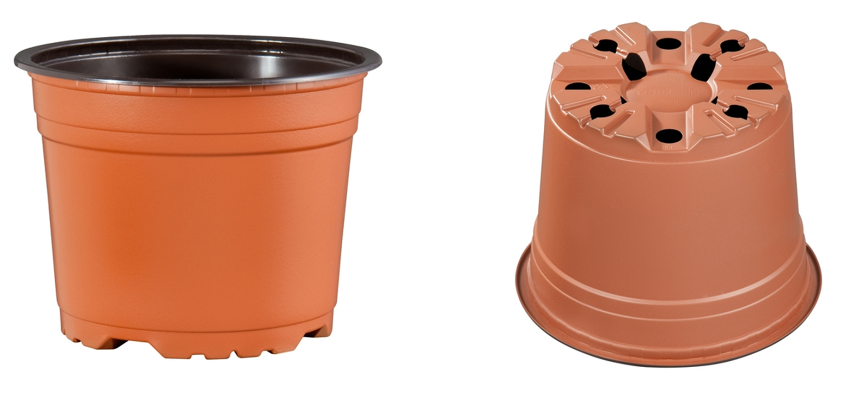
\includegraphics[width=0.7\textwidth]{Illustrationen/4-Entwurf/VCD_Serie.png}
	\caption{Pöppelmann VCD Serie}
	\label{fig:toepfe}
\end{figure}

Von substanzieller Bedeutung ist auch die verwendete Pflanzenerde. Da Erde von minderer Qualität eine hohe Menge an Fremdkörper wie Gehölz und Lehm enthalten kann. Die im Zusammenhang mit diesem Projekt verwendete Topferde ist deshalb auf die Artikel Nr.: 181 000 00 vom Hersteller RICOTER spezifiziert.

\subsection{Anforderungen}
\textit{(pro)} Die in diesem Unterkapitel ausgehandelten Anforderungen an den Planting Robot dienen zur Abgrenzung des Funktionsumfangs des Projekts. Weiter sollen sie dem Industriepartner eine genaue Vorstellung darüber bieten was er von dem fertigen Funktionsmuster erwarten kann.\\
\newline
Der Planting Robot soll stationär, auf dem Boden, neben der Topfmaschine platziert werden. Um einen präzisen Eingriff in die Produktionskette der Topfmaschine gewährleisten zu können, soll er an der Topfmaschine fixiert werden können. Der Planting Robot muss direkt am Topfkranz positioniert werden. Weiter soll der Planting Robot mit 230V Netzspannung ohne weitere Anschlüsse (z.B. Pressluft) betrieben werden können. Da der Planting Robot ein Funktionsmuster darstellt soll er nur für räumlichen Umgebungsbedingungen ausgelegt werden. \\
\newline
Der Setzprozess soll nur ausgeführt werden, wenn sich ein Topf in Position befindet. Drei Nemacaps sollen in einem Kreis mit einem Radius von 60$\%$ der Topfgrösse, mit einem Winkelabstand von jeweils 120° in den Topf eingesetzt werden (siehe Abb. \ref{fig:Setzprozess}). Dabei soll die Einsetztiefe variabel verstellbar sein, aber maximal 60$\%$ der Topfhöhe Betragen. 

\begin{figure}[H]
	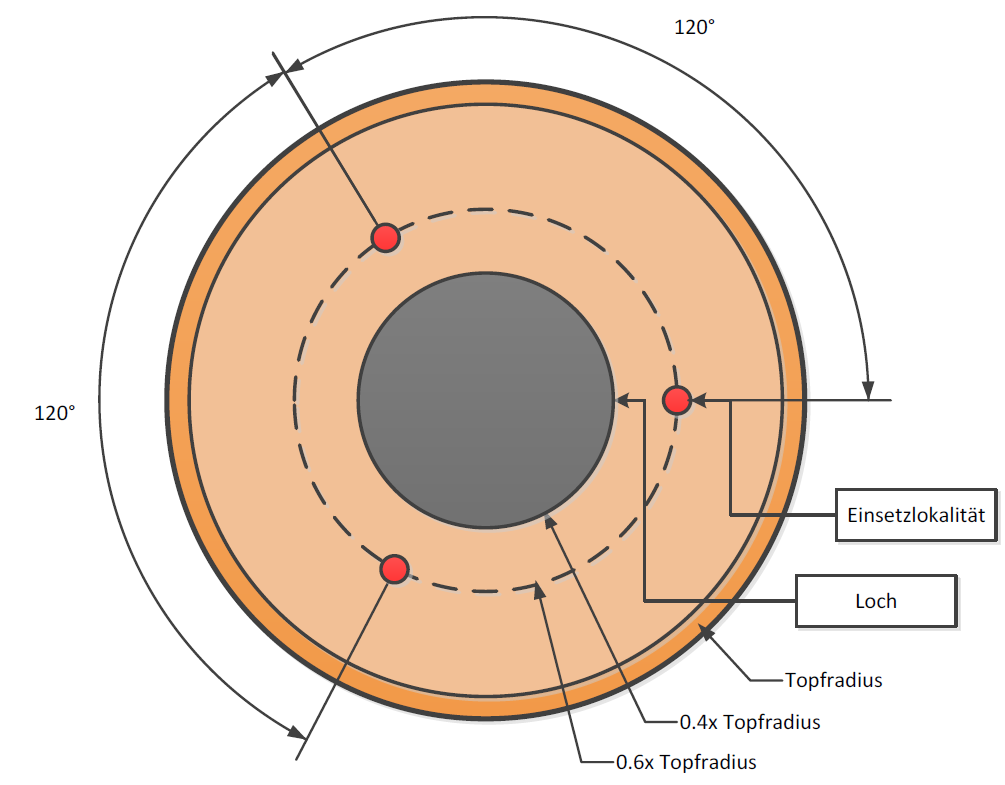
\includegraphics[width=0.6\textwidth]{Illustrationen/4-Entwurf/Setzprozess.png}
	\caption{Setzlokalität}
	\label{fig:Setzprozess}
\end{figure}

Während eines Produktionsbatches soll sich die Topfgrösse nicht ändern. Beim Wechsel auf einen neuen Batch mit anderer Topfgrösse soll der Planting Robot umkonfiguriert werden. Eine Wunschanforderung ist es, dass sich der Planting Robot automatisch auf einen Wechsel der Topfgrösse konfiguriert. Die Setzkadenz des Planting Robots soll mit der normalen Betriebsgeschwindigkeit der Topfmaschine TC2 mithalten können. Demnach sollen 2800 Töpfe pro Stunde mit Nemacaps bestückt werden können. Wunschanforderung ist eine Produktionskapazität von 3600 Töpfen pro Stunde. Dabei ist zu beachten, dass die Eingriffszeit des Planting Robots aufgrund der Stopp and Go Bewegung des Topfkranzes nur 50$\%$ beträgt.